\chapter[Dynamic partitioning for SMR]{Dynamic partitioning for SMR}
\label{sec:dssmr}
% \section{Limitation of static partitioned SMR} \label{sec:ssmrproblem}

An inherent problem of traditional SMR is that it is not scalable: any replica
added to the system will deliver all requests, so throughput is not increased.
Scalable SMR addresses this issue in two ways: (i) by partitioning the
application state, while allowing every command to access (read/write) any
combination of partitions and (ii) using caching to reduce the communication
across partitions, while keeping the execution linearizable.

On the downside of this approach, as the number of multi-partition commands
increases, performance of \ssmr\ becomes worse, as partitions must communicate.
One way to reduce the number of multi-partition commands is by dynamically
changing the partitioning, putting variables that are usually accessed together
in the same partition. However, the partitioning oracle of \ssmr\ relies on a
static mapping of variables to partitions. One advantage of this implementation
is that all clients and servers can have their own local oracle, which always
returns a correct set of partitions for every query. Such a static mapping has
the major limitation of not allowing the service to dynamically adapt to
different access patterns. Any state reorganization requires system shutdown and
manual intervention.

Given these issues, it is crucial that highly available partitioned systems be
able to dynamically adapt to the workload. In this section, we present
\dssmrlong\ (\dssmr), a technique that allows a partitioned SMR system to scale
by reconfiguring its data placement on-the-fly.

\section{\dssmrlong}
\label{sec:dssmridea}

Dynamic \ssmr\ (\dssmr) defines a dynamic mapping of variables to partitions.
Each variable $v$ is mapped to partition $\ppm$, meaning that $v \in \ppm$. Such
a mapping is managed by a partitioning oracle, which is implemented as a
replicated service run by a group of server processes $\ssm_0$. The oracle
service allows the mapping of variables to partitions to be retrieved or changed
during execution. In more detail, \dssmr\ distinguishes five types of commands:
$access(\omega)$ is an application command that accesses (reads or writes)
variables in set $\omega \subseteq \vvm$ (as described in
Section~\ref{sec:sysmodel}), $create(v)$ creates a new variable $v$ and
initially maps it to a partition defined by the oracle, $delete(v)$ removes $v$
from the service state,
% resulting in $part(v) = \emptyset$,
$move(v,\ppm_s,\ppm_d)$ moves variable $v$ from partition $\ppm_s$ to partition
$\ppm_d$, and $consult(C)$ asks the oracle which variables are accessed by
command $C$, and which partition contains each of them. The reply from the
oracle to a $consult$ command is called a $prophecy$. A prophecy usually
consists of a set of tuples $\langle v, \ppm \rangle$, meaning that variable $v$
is mapped to partition $\ppm$. The other possible values for a prophecy are $ok$
and $nok$, which mean that a command can and cannot be executed, respectively.

Clients can consult the oracle to know which partitions each command should be
multicast to, based on which variables are accessed by the command. If the reply
received from the oracle tells the client that the command accesses a single
partition, the client multicasts the command to that partition. If the command
accesses variables from multiple partitions, the client first multicasts one or
more $move$ commands to the oracle and to the involved partitions, with the
intent of having all variables in the same partition. Then, the command itself
is multicast to the one partition that now holds all variables accessed by the
command. If a subsequent command accesses the same variables, it will also
access a single partition. With this scheme, the access patterns of commands
will shape the mapping of variables to partitions, reducing the number of
multi-partition commands.

\begin{figure*}
\begin{minipage}[b]{1.0\linewidth} % A minipage that covers the whole width of
the page
\centering
      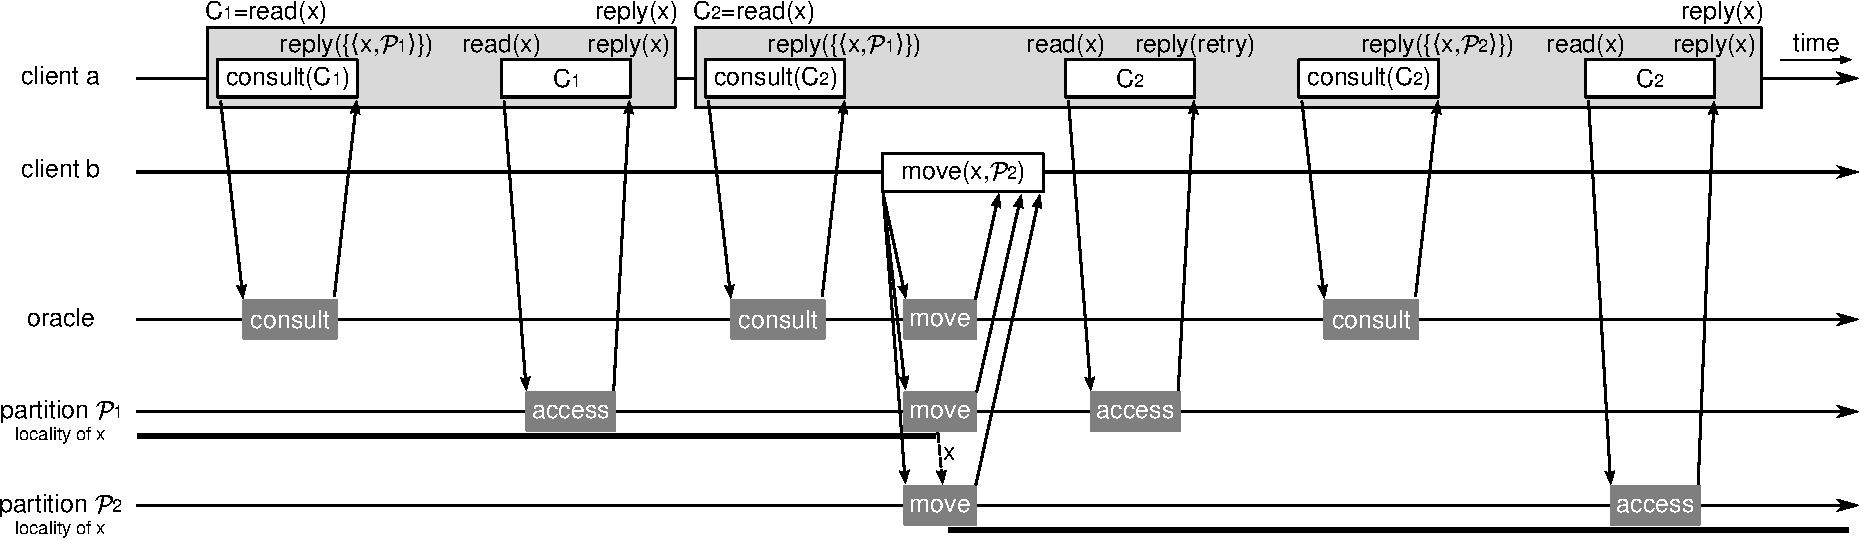
\includegraphics[width=0.8\linewidth]{figures/move_case_1}
\end{minipage}
\caption{Consulting the oracle and issuing a command are done in multiple calls to atomic-multicast.}
\label{fig:move_case_1}
\end{figure*}

Consulting the oracle and issuing the application command are done with separate
calls to atomic multicast in \dssmr{}. It may happen that, between those
operations, the partitioning changes. We illustrate this in
Figure~\ref{fig:move_case_1}. Commands $C_1$ and $C_2$ read variable $x$. Since
partitioning is dynamic, the client issuing the commands first consults the
oracle before multicasting each command. $C_1$ executes without the interference
of other commands, so consulting the oracle and multicasting the command only
once is enough for $C_1$ to be executed. However, before $C_2$ is multicast to
$\ppm_1$, another client issues a $move$ command that relocates $x$ to $\ppm_2$.
When $C_2$ is delivered at the servers of $\ppm_1$, the command is not executed,
since $x$ is not available at $\ppm_1$ anymore. A similar situation may arise
when a command accesses variables from multiple partitions, as it consists of
multicasting at least three commands separately: $consult$, $move$ and $access$.
The partitioning can change between the execution of any two of those commands.

To solve this problem, the client multicasts the set of variables accessed along
with each access command. Upon delivery, each server checks the set of variables
sent by the client. If all variables in the set belong to the local partition,
the command is executed; otherwise, a $retry$ message is sent back to the
client. When the client receives a $retry$ message, it consults the oracle
again, possibly moving variables across partitions, and then reissues the access
command. To guarantee termination, if the command fails a certain number of
times, the client multicasts the command to all partitions and the servers
execute it as in the original \ssmr{}.

\section{Optimizations}
\label{sec:optm}

\textbf{Caching.} For every command, the client consults the oracle. If every
command passes by the oracle, the system is unlikely to scale, as the oracle is
prone to becoming a bottleneck. To provide a scalable solution, each client has
a local cache of the partitioning information. Before multicasting an
application command $C$ to be executed, the client checks whether the cache has
information about every variable concerned by $C$. If the cache does have such
knowledge, the oracle is not consulted and the information contained in the
cache is used instead. If the reply to $C$ is $retry$, the oracle is consulted
and the returned prophecy is used to update the client's cache. The cache is a
local service that follows an algorithm similar to that of the oracle, except it
responds only to $consult(C)$ commands and, in situations where the oracle would
return $ok$ or $nok$, the cache tells the client to consult the actual oracle.

Naturally, the cached partitioning information held by the client may be out of
date. This may lead a command to be multicast to the wrong set of partitions,
which will probably incur in the client having to retry the command.
%For instance, in Figure~\ref{fig:cache_retry} the client has an out-of-date
%cache, incurring in a new consultation to the oracle when executing $C_3$. On
%the other hand, the client may already have to retry commands, even if the
%oracle is always consulted first, as shown in Figure~\ref{fig:move_case_1}.
If most commands are executed without consulting the oracle, we avoid turning
the oracle into a bottleneck. Moreover, such a cache can be updated ahead of
time, not having to wait for an actual application command to be issued to only
then consult the oracle. This way, the client can keep a cache of partitioning
information of variables that the client deems likely to be accessed in the
future.

%\begin{figure*} \begin{minipage}[b]{1\linewidth} % A minipage that covers the
%whole width of the page \centering
%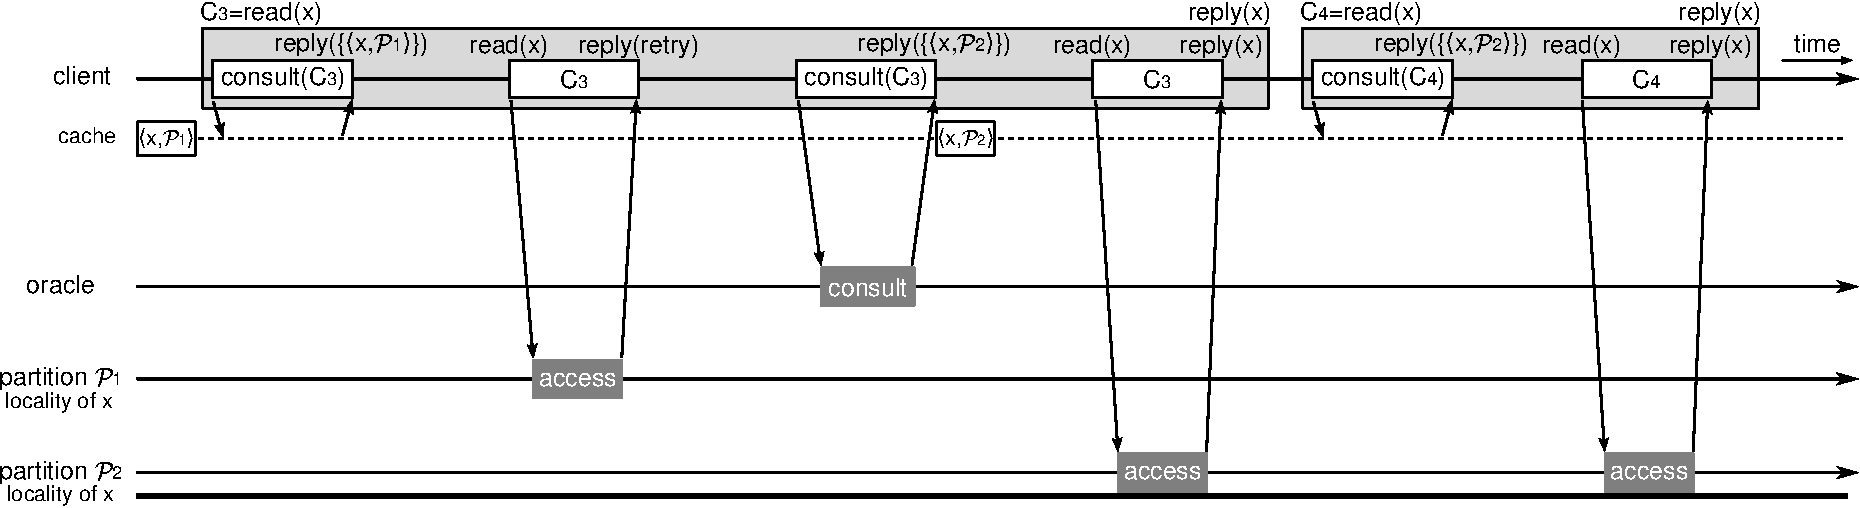
\includegraphics[width=1.0\linewidth]{figures/cache_retry} \end{minipage}
%\caption{Each client in \dssmr\ maintains a cache in order to avoid  consulting
%the oracle. White boxes represent actions of the client proxy.}
%\label{fig:cache_retry} \end{figure*}

\textbf{Load balancing}. When moving variables, the client may try to distribute
them in a way that balances the workload among partitions. This way, the system
is more likely to scale throughput with the number of server groups. One way of
balancing load is by having roughly the same number of state variables in every
partition. This can be implemented by having client choose randomly the
partition that will receive all variables concerned by each command. Besides
improving performance, balancing the load among partitions prevents the system
from degenerating into a single-partition system, with all variables moved to
the same place as commands are executed.

% \section{Correctness} \label{sec:correctness}

% In this section, we argue that \dssmr\ ensures termination and
% linearizability. By ensuring termination, we mean that for every command $C$
% issued by a correct client, a reply to $C$ different than $retry$ is
% eventually received by the client. This assumes that at least one oracle
% process is correct and that every partition has at least one correct server.
% Given these constraints, the only thing that could prevent a command from
% terminating would be an execution that forced the client proxy to keep
% retrying a command. This problem is trivially solved by falling back to \ssmr\
% after a predefined number of retries: at a certain point, the client proxy
% multicast the command to all server and oracle processes, which execute the
% command as in \ssmr{}, i.e., with coordination among all partitions and the
% oracle.

% As for linearizability, we argue that, if every command in execution \ex\ of
% \dssmr\ is delivered by atomic multicast and is \emph{execution atomic} (as
% defined in~\cite{bezerra2014ssmr}), then \ex\ is linearizable. We denote the
% order given by atomic multicast by relation $\prec$. Given any two messages
% $m_1$ and $m_2$, ``$m_1 \prec m_2$'' means that there exists a process that
% delivers both messages and $m_1$ is delivered before $m_2$, or there is some
% message $m'$ such that $m_1 \prec m'$ and $m' \prec m_2$, which can be written
% as \mbox{$m_1 \prec m' \prec m_2$}. %\fxnote[draft]{use the phrase \"there
% exists a process that\" } Also, for the purposes of this proof, we consider
% the oracle to be a partition, as it also \amdel{}s and executes application
% commands.

% Suppose, by means of contradiction, that there exist two commands $x$ and $y$,
% where $x$ finishes before $y$ starts, but $y \prec x$ in the execution. There
% are two possibilities to be considered: (i) $x$ and $y$ are delivered by the
% same process $p$, or (ii) no process delivers both $x$ and $y$.

% In case (i), at least one process $p$ delivers both $x$ and $y$. As $x$
% finishes before $y$ starts, then $p$ delivers $x$, then $y$. From the
% properties of atomic multicast, and since each partition is mapped to a
% multicast group, no process delivers $y$, then $x$. Therefore, we reach a
% contradiction in this case.

% In case (ii), if there were no other commands in \ex, then the execution of
% $x$ and $y$ could be done in any order, which would contradict the supposition
% that $y \prec x$. Therefore, there are commands $z_1, ..., z_n$ with atomic
% order $y \prec z_1 \prec \cdots \prec z_n \prec x$, where some process $p_0$
% (of partition $\ppm_0$) delivers $y$, then $z_1$; some process $p_1 \in
% \ppm_1$ delivers $z_1$, then $z_2$, and so on: process $p_i \in \ppm_i$
% delivers $z_{i}$, then $z_{i+1}$, where $1 \leq i < n$. Finally, process $p_n
% \in \ppm_n$ delivers $z_n$, then $x$.

% Let $z_0 = y$ and let $atomic(i)$ be the following predicate: ``For every
% process $p_i \in \ppm_i$, $p_i$ finishes executing $z_i$ only after some $p_0
% \in \ppm_0$ started executing $z_0$.'' We now claim that $atomic(i)$ is true
% for every $i$, where $0 \leq i \leq n$. We prove our claim by induction.

% %\begin{itemize}

% %\item \emph{Basis ($i=0$)}: $atomic(0)$ is obviously true, as $p_0$ can only
% finish executing $z_0$ after starting executing it.

% %\item \emph{Induction step}: If $atomic(i)$, then $atomic(i+1)$.
% \\
% Proof: Command $z_{i+1}$ is multicast to both $\ppm_i$ and $\ppm_{i+1}$. Since
% $z_{i+1}$ is execution atomic, before any $p_{i+1} \in \ppm_{i+1}$ finishes
% executing $z_{i+1}$, some $p_i \in \ppm_i$ starts executing $z_{i+1}$. Since
% $z_i \prec z_{i+1}$, every $p_i \in \ppm_i$ start executing $z_{i+1}$ only
% after finishing the execution of $z_i$. As $atomic(i)$ is true, this will only
% happen after some $p_0 \in \ppm_0$ started executing $z_0$.

% %\end{itemize}

% As $z_n \prec x$, for every $p_n \in \ppm_n$, $p_n$ executes command $x$ only
% after the execution of $z_n$ at $p_n$ finishes. From the above claim, this
% happens only after some $p_0 \in \ppm_0$ starts executing $y$. This means that
% $y$ ($z_0$) was issued by a client before any client received a response for
% $x$, which contradicts the assumption that $x$ precedes $y$ in real-time,
% i.e., that command $y$ was issued after the reply for command $x$ was
% received.

\section{Conclusion}
\label{sec:dssmnr-conclusion}
This chapter introduced \dssmr, the initial idea of \dynastar. So far, we have
proposed an approach that allows scaling state-machine replication by
dynamically repartitioning application state based on the workload.  Variables
that are usually accessed together are moved to the same partition, which
significantly improves scalability. However, in order to reduce the chances of
skewed load among partitions in \dssmr\, the destination partition is chosen
randomly. Although this heuristic algorithm could bring a balanced partitioning,
it fails to guarantee optimal partitioning and to minimize the rate of
multi-partition commands. In the next chapter, we will discuss more details
about reaching an optimized partitioning. More details, including a proof of
correctness and performance evaluation of \dssmr{} is available in
\cite{le2016dssmr}
